\documentclass[12pt,a4paper]{article}

\usepackage{fontspec}
\usepackage[vietnamese]{babel}
\setmainfont{Times New Roman}
\setsansfont{Arial}
\setmonofont{Consolas}
\usepackage{geometry}
\usepackage{graphicx}
\usepackage{float}
\usepackage{booktabs}
\usepackage{array}
\usepackage{xcolor}
\usepackage{listings}
\usepackage{longtable}
\usepackage{hyperref}
\usepackage{amsmath}

\geometry{
    left=2.5cm,
    right=2.0cm,
    top=2.0cm,
    bottom=2.0cm
}

\hypersetup{
    colorlinks=true,
    linkcolor=blue,
    urlcolor=blue
}

\lstdefinestyle{cppstyle}{
    language=C++,
    basicstyle=\ttfamily\small,
    keywordstyle=\color{blue},
    commentstyle=\color{gray},
    stringstyle=\color{red!60!black},
    numbers=left,
    numberstyle=\tiny,
    stepnumber=1,
    frame=single,
    breaklines=true,
    tabsize=4,
    showstringspaces=false
}

\begin{document}

% ==================================================
% TRANG BIA
% ==================================================

\begin{titlepage}
    \centering
    {\Large \textbf{TRƯỜNG: \underline{\hspace{8cm}}}}\\[0.5cm]
    {\Large \textbf{KHOA / VIỆN: \underline{\hspace{7cm}}}}\\[3cm]

    {\LARGE \textbf{BÁO CÁO BÀI TẬP LỚN}}\\[0.5cm]
    {\Large \textbf{Đề tài: Chương trình thi trắc nghiệm đơn giản}}\\[0.5cm]
    {\large Ngôn ngữ lập trình: C++}\\[3cm]

    \begin{flushleft}
        \textbf{Môn học:} Kỹ thuật lập trình\\[0.3cm]
        \textbf{Nhóm thực hiện:} Nhóm 3\\[0.3cm]
        \textbf{Lớp:} \underline{\hspace{6cm}}\\[0.3cm]
        \textbf{Giảng viên hướng dẫn:} \underline{\hspace{6cm}}\\[0.8cm]
    \end{flushleft}

    \begin{center}
    \begin{tabular}{|c|p{6cm}|p{5cm}|}
        \hline
        \textbf{STT} & \textbf{Họ và tên} & \textbf{MSSV} \\
        \hline
        1 & \underline{\hspace{5.5cm}} & \underline{\hspace{4.5cm}} \\
        \hline
        2 & \underline{\hspace{5.5cm}} & \underline{\hspace{4.5cm}} \\
        \hline
        3 & \underline{\hspace{5.5cm}} & \underline{\hspace{4.5cm}} \\
        \hline
    \end{tabular}
    \end{center}

    \vfill
    {\large Hà Nội, \today}
\end{titlepage}

\tableofcontents
\newpage

% ==================================================
% 1. THONG TIN THUC HIEN
% ==================================================

\section{Thông tin người thực hiện và phân công}

Bài tập lớn được thực hiện theo nhóm 3 sinh viên. Mỗi thành viên phụ trách một nhóm chức năng chính để đảm bảo chương trình được chia việc rõ ràng và dễ kiểm soát.

\begin{table}[H]
\centering
\begin{tabular}{|c|p{5cm}|p{8cm}|}
\hline
\textbf{STT} & \textbf{Thành viên} & \textbf{Phân công công việc} \\
\hline
1 & Sinh viên 1 & Phụ trách \texttt{du\_lieu.h} và \texttt{du\_lieu.cpp}: thiết kế cấu trúc dữ liệu, tổ chức danh sách bằng \texttt{vector}, hàm tiện ích, đọc/ghi file dữ liệu. \\
\hline
2 & Sinh viên 2 & Phụ trách \texttt{ngan\_hang\_cau\_hoi.h} và \texttt{ngan\_hang\_cau\_hoi.cpp}: xây dựng ngân hàng câu hỏi, thêm/xem câu hỏi theo học phần. \\
\hline
3 & Sinh viên 3 & Phụ trách \texttt{thi\_bao\_cao.h} và \texttt{thi\_bao\_cao.cpp}: sinh đề, làm bài thi, chấm điểm, báo cáo kết quả và menu chính. \\
\hline
\end{tabular}
\caption{Bảng phân công công việc nhóm}
\end{table}

% ==================================================
% 2. MO TA TONG THE
% ==================================================

\section{Mô tả tổng thể chương trình}

Chương trình được xây dựng bằng ngôn ngữ C++ dưới dạng ứng dụng console. Mục tiêu của chương trình là hỗ trợ tổ chức một bài thi trắc nghiệm đơn giản, bao gồm quản lý ngân hàng câu hỏi, cấu hình đề thi, làm bài, chấm điểm tự động và xem báo cáo kết quả nhiều lần thi.

\subsection{Các chức năng chính}

Các chức năng chính của chương trình gồm:

\begin{itemize}
    \item Quản lý ngân hàng câu hỏi theo môn học/học phần.
    \item Mỗi câu hỏi có nội dung, 4 đáp án, đáp án đúng và mức độ khó.
    \item Cấu hình đề thi bằng cách chọn môn học, số câu hỏi dễ, số câu hỏi khó và thời gian làm bài.
    \item Sinh đề thi ngẫu nhiên bằng cách xáo trộn thứ tự câu hỏi.
    \item Xáo trộn thứ tự đáp án trong từng câu hỏi.
    \item Cho thí sinh làm bài trên giao diện console.
    \item Tính thời gian làm bài và tự động thu bài khi hết giờ.
    \item Chấm điểm tự động theo số câu trả lời đúng.
    \item Lưu và hiển thị báo cáo kết quả của nhiều lần thi.
\end{itemize}

\subsection{Phạm vi chương trình}

Do đây là bài tập lớn ở mức sinh viên đại học, chương trình tập trung vào các chức năng cốt lõi thay vì xây dựng hệ thống hoàn chỉnh như phần mềm thực tế. Các chức năng nâng cao như đăng nhập, phân quyền, giao diện đồ họa, sửa/xóa chi tiết nhiều loại dữ liệu không được triển khai để giữ chương trình đơn giản, dễ hiểu và dễ bảo vệ.

% ==================================================
% 3. THIET KE VA TO CHUC CHUONG TRINH
% ==================================================

\section{Thiết kế và tổ chức chương trình}

Chương trình được tách thành nhiều file theo nhóm chức năng để phù hợp với cách làm việc nhóm. File \texttt{main.cpp} chỉ còn nhiệm vụ khởi động chương trình, còn các phần xử lý chính được đặt trong các file riêng để 3 thành viên có thể làm việc độc lập hơn.

\begin{table}[H]
\centering
\begin{tabular}{|p{4cm}|p{10cm}|}
\hline
\textbf{File} & \textbf{Nội dung phụ trách} \\
\hline
\texttt{du\_lieu.h} & Khai báo hằng số, \texttt{struct}, biến toàn cục và nguyên mẫu các hàm dữ liệu/tiện ích. \\
\hline
\texttt{du\_lieu.cpp} & Cài đặt hàm tiện ích, đọc/ghi file, tìm kiếm môn học, thí sinh và câu hỏi. \\
\hline
\texttt{ngan\_hang\_cau\_hoi.h/.cpp} & Cài đặt chức năng hiển thị môn học, xem câu hỏi, thêm câu hỏi và đếm câu hỏi theo độ khó. \\
\hline
\texttt{thi\_bao\_cao.h/.cpp} & Cài đặt sinh đề, làm bài, tính giờ, chấm điểm, lưu kết quả, báo cáo và menu chính. \\
\hline
\texttt{main.cpp} & Gọi hàm đọc dữ liệu, mở menu chính và kết thúc chương trình. \\
\hline
\end{tabular}
\caption{Tổ chức file chương trình sau khi tách module}
\end{table}

\subsection{Các nhóm hàm chính}

\begin{longtable}{|p{5cm}|p{9cm}|}
\hline
\textbf{Nhóm hàm} & \textbf{Vai trò} \\
\hline
\texttt{vector} & Lưu danh sách môn học, câu hỏi, thí sinh và kết quả thi. \\
\hline
Hàm tiện ích & Nhập dữ liệu, xử lý chuỗi, tách dòng file, lấy thời gian hiện tại, xáo trộn mảng. \\
\hline
Đọc/ghi file & Đọc dữ liệu từ file text khi mở chương trình và ghi lại dữ liệu khi thoát hoặc có thay đổi. \\
\hline
Ngân hàng câu hỏi & Hiển thị học phần, xem câu hỏi theo học phần, thêm câu hỏi mới. \\
\hline
Thi trắc nghiệm & Chọn thí sinh, chọn môn học, cấu hình số câu hỏi và thời gian, sinh đề và làm bài. \\
\hline
Chấm điểm và báo cáo & Đếm số câu đúng, tính điểm, lưu kết quả, hiển thị báo cáo nhiều lần thi. \\
\hline
Menu chính & Điều hướng người dùng đến các chức năng chính. \\
\hline
\end{longtable}

\subsection{Các cấu trúc dữ liệu chính}

Chương trình sử dụng các \texttt{struct} sau:

\begin{itemize}
    \item \texttt{MonHoc}: lưu mã môn học và tên môn học.
    \item \texttt{CauHoi}: lưu nội dung câu hỏi, 4 đáp án, đáp án đúng và mức độ.
    \item \texttt{ThiSinh}: lưu mã thí sinh và họ tên.
    \item \texttt{CauHoiThi}: lưu câu hỏi trong đề thi, thứ tự đáp án sau khi xáo trộn và đáp án đã chọn.
    \item \texttt{KetQuaThi}: lưu kết quả của một lần thi.
\end{itemize}

\subsection{Tổ chức menu}

Menu chính của chương trình gồm 3 nhóm chức năng:

\begin{enumerate}
    \item Quản lý ngân hàng câu hỏi.
    \item Cấu hình đề thi theo số câu dễ/khó và bắt đầu thi.
    \item Báo cáo kết quả thi.
\end{enumerate}

\begin{figure}[H]
    \centering
    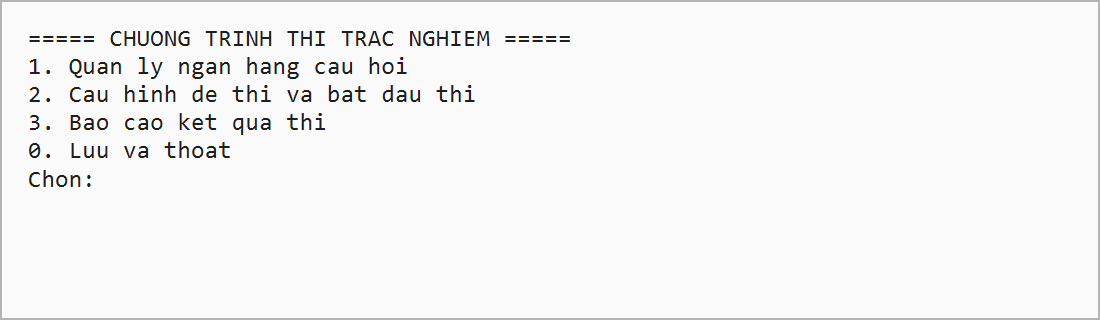
\includegraphics[width=0.9\textwidth]{report_assets/menu_chinh.png}
    \caption{Giao diện menu chính của chương trình}
\end{figure}

% ==================================================
% 4. FILE DU LIEU
% ==================================================

\section{Tổ chức file dữ liệu}

Dữ liệu của chương trình được lưu bằng file text. Mỗi dòng trong file là một bản ghi, các trường được phân tách bằng ký tự \texttt{|}.

\begin{table}[H]
\centering
\begin{tabular}{|p{4cm}|p{10cm}|}
\hline
\textbf{File} & \textbf{Ý nghĩa} \\
\hline
\texttt{subjects.txt} & Lưu danh sách môn học/học phần. \\
\hline
\texttt{questions.txt} & Lưu ngân hàng câu hỏi trắc nghiệm. \\
\hline
\texttt{candidates.txt} & Lưu danh sách thí sinh. \\
\hline
\texttt{results.txt} & Lưu kết quả các lần thi. \\
\hline
\end{tabular}
\caption{Các file dữ liệu của chương trình}
\end{table}

\subsection{Bộ dữ liệu mẫu sử dụng khi kiểm thử}

Bộ dữ liệu mẫu được rút gọn ở mức vừa đủ để kiểm thử và trình bày trong báo cáo. Dataset không quá lớn, giúp việc chạy chương trình trên console dễ quan sát hơn, nhưng vẫn đủ dữ liệu cho chức năng sinh đề theo số câu dễ và số câu khó.

\begin{table}[H]
\centering
\begin{tabular}{|p{4cm}|p{3cm}|p{7cm}|}
\hline
\textbf{File} & \textbf{Số dòng} & \textbf{Ghi chú} \\
\hline
\texttt{subjects.txt} & 5 & Danh sách 5 môn học/học phần. \\
\hline
\texttt{candidates.txt} & 12 & Danh sách thí sinh mẫu. \\
\hline
\texttt{questions.txt} & 50 & Mỗi môn có 10 câu hỏi, gồm 5 câu dễ và 5 câu khó. \\
\hline
\texttt{results.txt} & 20 & Kết quả mẫu của nhiều lần thi. \\
\hline
\end{tabular}
\caption{Thống kê bộ dữ liệu mẫu sau khi rút gọn}
\end{table}

\subsection{Định dạng file}

\begin{lstlisting}[style=cppstyle, caption={Định dạng dữ liệu text}]
subjects.txt:
maMonHoc|tenMonHoc

questions.txt:
maCauHoi|maMonHoc|mucDo|noiDung|dapAnA|dapAnB|dapAnC|dapAnD|dapAnDung

candidates.txt:
maThiSinh|hoTen

results.txt:
maKetQua|maThiSinh|maMonHoc|tongSoCau|soCauDung|thoiGianThi|thoiGianLamBaiGiay
\end{lstlisting}

Trong file \texttt{results.txt}, chương trình không lưu trực tiếp trường điểm vì điểm có thể tính lại từ \texttt{soCauDung} và \texttt{tongSoCau}. Cách này giúp dữ liệu gọn hơn và tránh trường hợp điểm lưu trong file không khớp với số câu đúng.

% ==================================================
% 5. LOGIC NGHIEP VU
% ==================================================

\section{Logic nghiệp vụ chính}

\subsection{Quản lý ngân hàng câu hỏi}

Ngân hàng câu hỏi được tổ chức theo môn học. Khi thêm câu hỏi, người dùng cần chọn mã môn học, nhập mức độ, nội dung câu hỏi, 4 đáp án và đáp án đúng. Chương trình kiểm tra mã môn học có tồn tại hay không trước khi thêm câu hỏi.

\begin{figure}[H]
    \centering
    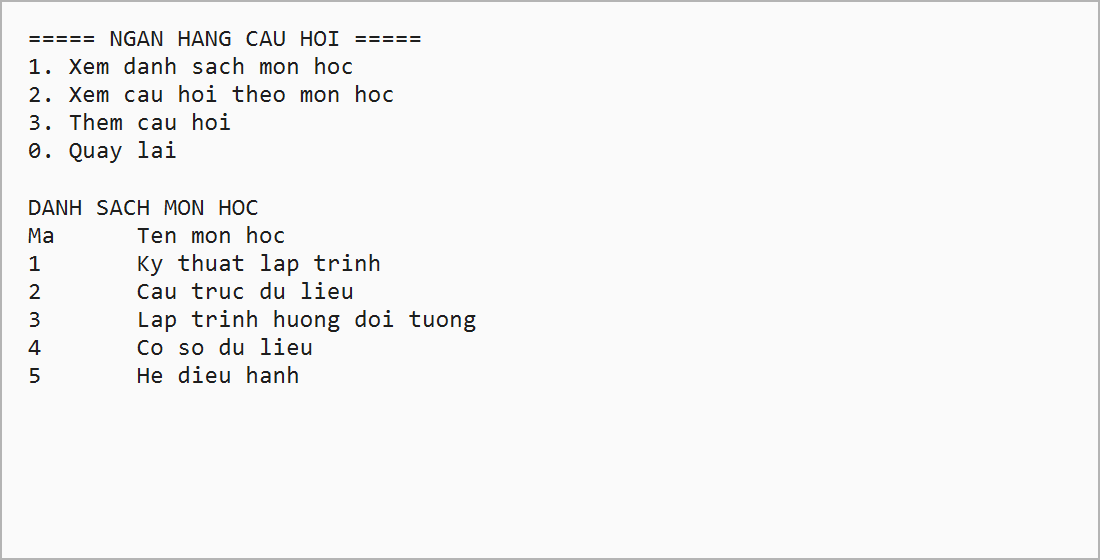
\includegraphics[width=0.9\textwidth]{report_assets/ngan_hang_cau_hoi.png}
    \caption{Giao diện quản lý ngân hàng câu hỏi}
\end{figure}

\subsection{Cấu hình và sinh đề thi}

Khi bắt đầu thi, chương trình yêu cầu nhập:

\begin{itemize}
    \item Mã thí sinh.
    \item Mã môn học.
    \item Số lượng câu hỏi dễ trong đề thi.
    \item Số lượng câu hỏi khó trong đề thi.
    \item Thời gian làm bài tính theo phút.
\end{itemize}

Sau đó chương trình lọc các câu hỏi theo môn học đã chọn và theo mức độ dễ/khó. Danh sách câu hỏi hợp lệ được xáo trộn bằng thuật toán Fisher-Yates. Chương trình lấy đúng số câu dễ và số câu khó theo cấu hình để tạo đề thi.

\subsection{Xáo trộn câu hỏi và đáp án}

Việc xáo trộn được áp dụng ở hai mức:

\begin{itemize}
    \item Xáo trộn thứ tự câu hỏi để mỗi lần thi có đề khác nhau.
    \item Xáo trộn thứ tự 4 đáp án trong từng câu hỏi để hạn chế học thuộc vị trí đáp án.
\end{itemize}

Khi thí sinh chọn đáp án A/B/C/D, chương trình ánh xạ đáp án hiển thị về chỉ số đáp án gốc để chấm điểm chính xác.

\subsection{Tính giờ và tự động thu bài}

Chương trình ghi nhận thời điểm bắt đầu làm bài bằng hàm \texttt{time(NULL)}. Trước mỗi câu hỏi, chương trình kiểm tra thời gian đã làm bài. Nếu thời gian vượt quá giới hạn, chương trình dừng bài thi và tự động chuyển sang phần chấm điểm.

\subsection{Chấm điểm và báo cáo}

Sau khi làm bài, chương trình đếm số câu trả lời đúng và tính điểm theo công thức:

\[
    \text{Điểm} = \frac{\text{Số câu đúng} \times 10}{\text{Tổng số câu}}
\]

Kết quả thi được lưu vào file \texttt{results.txt}. Mỗi lần thi tạo ra một bản ghi mới để có thể xem báo cáo kết quả nhiều lần thi. Trường điểm không lưu trực tiếp trong file mà được tính lại khi đọc dữ liệu hoặc khi hiển thị báo cáo.

\begin{figure}[H]
    \centering
    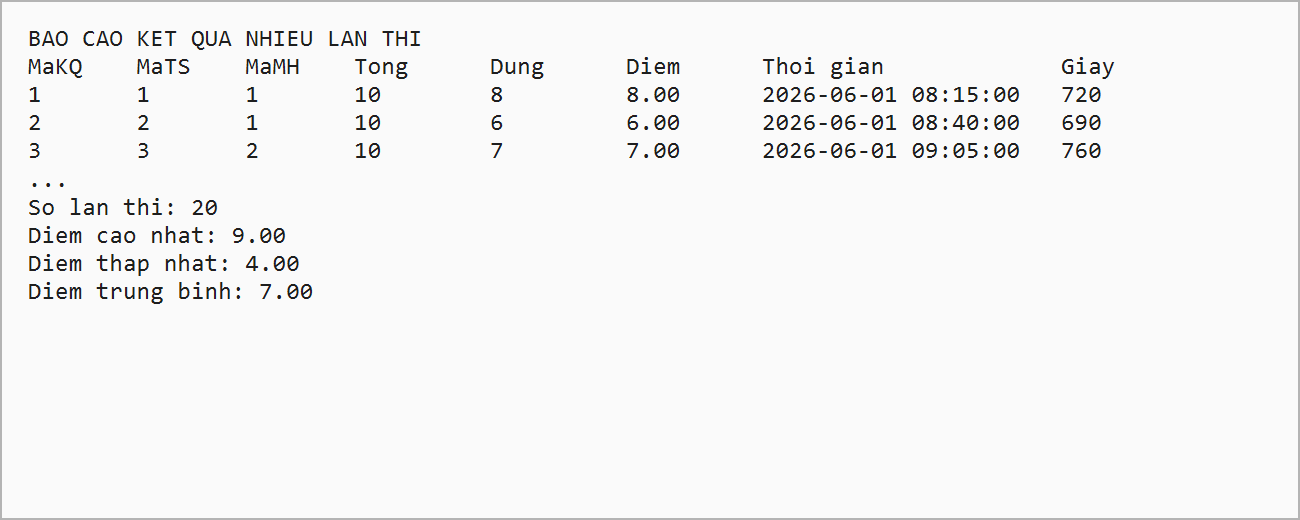
\includegraphics[width=0.95\textwidth]{report_assets/bao_cao_ket_qua.png}
    \caption{Báo cáo kết quả nhiều lần thi}
\end{figure}

% ==================================================
% 6. KIEM THU
% ==================================================

\section{Đánh giá và kiểm thử chương trình}

\subsection{Mục tiêu và phương pháp kiểm thử}

Việc kiểm thử được thực hiện nhằm xác nhận chương trình đáp ứng đúng các yêu cầu chính của đề tài: đọc/ghi dữ liệu, quản lý ngân hàng câu hỏi, sinh đề theo số câu dễ/khó, làm bài có tính giờ, chấm điểm tự động và hiển thị báo cáo kết quả.

Nhóm sử dụng hai cách kiểm thử:

\begin{itemize}
    \item Kiểm thử theo chức năng: chạy chương trình trên console và thao tác theo từng menu.
    \item Kiểm thử chương trình con: kiểm tra riêng một số hàm quan trọng bằng dữ liệu đầu vào cụ thể và so sánh với kết quả mong đợi.
\end{itemize}

\subsection{Kiểm thử theo chức năng}

\begin{table}[H]
\centering
\begin{tabular}{|c|p{4.4cm}|p{4.4cm}|p{3.2cm}|p{1.4cm}|}
\hline
\textbf{STT} & \textbf{Tình huống kiểm thử} & \textbf{Dữ liệu thao tác} & \textbf{Kết quả thực tế} & \textbf{Đánh giá} \\
\hline
1 & Mở chương trình khi đã có file dữ liệu & Chạy file \texttt{thi\_trac\_nghiem.exe} & Đọc được môn học, câu hỏi, thí sinh, kết quả & Đạt \\
\hline
2 & Xem danh sách môn học & Chọn menu ngân hàng câu hỏi & Hiển thị đúng 5 học phần trong \texttt{subjects.txt} & Đạt \\
\hline
3 & Thêm câu hỏi mới hợp lệ & Nhập đủ nội dung, 4 đáp án, đáp án đúng và mức độ & Câu hỏi được thêm vào vector và lưu xuống file & Đạt \\
\hline
4 & Thêm câu hỏi với mã môn học sai & Nhập mã môn học không có trong danh sách & Chương trình báo lỗi và không thêm câu hỏi & Đạt \\
\hline
5 & Sinh đề theo số câu dễ/khó & Chọn môn 1, 2 câu dễ, 2 câu khó & Đề thi có 4 câu và đúng cơ cấu dễ/khó & Đạt \\
\hline
6 & Nhập đáp án không hợp lệ & Nhập ký tự ngoài A, B, C, D & Chương trình yêu cầu nhập lại, không ghi nhận đáp án sai định dạng & Đạt \\
\hline
7 & Làm bài và nộp bài & Chọn đáp án cho từng câu rồi nộp & Chấm điểm tự động và lưu kết quả vào \texttt{results.txt} & Đạt \\
\hline
8 & Hết thời gian làm bài & Cấu hình thời gian ngắn để kiểm tra & Chương trình tự động thu bài khi hết giờ & Đạt \\
\hline
9 & Xem báo cáo kết quả & Chọn menu báo cáo kết quả & Hiển thị nhiều lần thi và điểm được tính lại từ số câu đúng & Đạt \\
\hline
\end{tabular}
\caption{Bảng kiểm thử theo chức năng}
\end{table}

\subsection{Kết quả thực hiện khi chạy chương trình}

Chương trình đã được biên dịch thành công bằng lệnh:

\begin{lstlisting}[style=cppstyle, caption={Lệnh biên dịch chương trình}]
g++ -std=c++11 -Wall -Wextra main.cpp du_lieu.cpp ngan_hang_cau_hoi.cpp thi_bao_cao.cpp -o thi_trac_nghiem.exe
\end{lstlisting}

Khi chạy thử với bộ dữ liệu mẫu, chương trình đọc được 4 file dữ liệu, hiển thị menu chính, cho phép xem ngân hàng câu hỏi, cấu hình đề thi, làm bài và xem báo cáo kết quả.

\begin{itemize}
    \item File \texttt{subjects.txt}: đọc được 5 môn học.
    \item File \texttt{questions.txt}: đọc được 50 câu hỏi, mỗi môn có 5 câu dễ và 5 câu khó.
    \item File \texttt{candidates.txt}: đọc được 12 thí sinh.
    \item File \texttt{results.txt}: đọc được 20 kết quả thi mẫu.
\end{itemize}

\subsection{Kiểm thử từng chương trình con tiêu biểu}

Do chương trình có nhiều hàm nhỏ, phần kiểm thử tập trung vào các chương trình con quan trọng và có ảnh hưởng trực tiếp đến logic nghiệp vụ. Các hàm tiện ích được kiểm thử thông qua dữ liệu đầu vào cụ thể, còn các hàm xử lý nghiệp vụ được kiểm thử bằng kết quả sinh đề, chấm điểm và báo cáo.

\begin{longtable}{|p{3.8cm}|p{4.1cm}|p{4.2cm}|p{2cm}|}
\hline
\textbf{Chương trình con} & \textbf{Dữ liệu kiểm thử} & \textbf{Kết quả mong đợi} & \textbf{Đánh giá} \\
\hline
\endfirsthead
\hline
\textbf{Chương trình con} & \textbf{Dữ liệu kiểm thử} & \textbf{Kết quả mong đợi} & \textbf{Đánh giá} \\
\hline
\endhead
\texttt{catKhoangTrang()} & Chuỗi \texttt{"  ABC  "} & Trả về \texttt{"ABC"} & Đạt \\
\hline
\texttt{laSoNguyen()} & \texttt{"123"}, \texttt{"12a"} & \texttt{true}, \texttt{false} & Đạt \\
\hline
\texttt{chuoiSangSo()} & \texttt{"10"}, \texttt{"7.5"} & Trả về \texttt{10} và \texttt{7.5} & Đạt \\
\hline
\texttt{tachDong()} & \texttt{"1|Ky thuat lap trinh"} & Tách được 2 trường & Đạt \\
\hline
\texttt{tinhDiem()} & \texttt{8/10}, \texttt{0/0} & Trả về \texttt{8.0}, \texttt{0} & Đạt \\
\hline
\texttt{xaoTronVectorSoNguyen()} & Vector \texttt{1,2,3,4} & Vẫn đủ 4 phần tử, thứ tự có thể thay đổi & Đạt \\
\hline
\texttt{demCauHoiTheoMonVaLoai()} & Môn 1, loại dễ và khó & Mỗi loại có 5 câu hỏi trong dataset mẫu & Đạt \\
\hline
\texttt{sinhDeThi()} & Môn 1, 2 câu dễ, 2 câu khó & Sinh đề có 4 câu, gồm đúng số câu dễ/khó & Đạt \\
\hline
\texttt{demCauDung()} & Đề thi có đáp án đã chọn & Đếm đúng số câu trùng đáp án đúng & Đạt \\
\hline
\texttt{hienThiBaoCaoKetQua()} & File \texttt{results.txt} có 20 kết quả & Hiển thị 20 dòng và thống kê điểm & Đạt \\
\hline
\caption{Kiểm thử các chương trình con tiêu biểu}
\end{longtable}

\subsection{Code kiểm thử minh họa}

Đoạn code sau được dùng để kiểm tra nhanh các hàm tiện ích và hàm tính điểm. Khi chạy kiểm thử, các giá trị in ra được đối chiếu với kết quả mong đợi trong bảng kiểm thử.

\begin{lstlisting}[style=cppstyle, caption={Code kiểm thử một số chương trình con}]
void kiemThuHamTienIch() {
    cout << catKhoangTrang("  ABC  ") << endl;
    cout << laSoNguyen("123") << endl;
    cout << laSoNguyen("12a") << endl;
    cout << chuoiSangSo("10") << endl;
    cout << chuoiSangSo("7.5") << endl;
    cout << tinhDiem(8, 10) << endl;
    cout << tinhDiem(0, 0) << endl;

    string truong[3];
    int soTruong = tachDong("1|Ky thuat lap trinh", truong, 3);
    cout << soTruong << endl;
    cout << truong[0] << " - " << truong[1] << endl;
}
\end{lstlisting}

Kết quả khi chạy đoạn kiểm thử trên:

\begin{lstlisting}[style=cppstyle, caption={Kết quả kiểm thử hàm tiện ích}]
ABC
1
0
10
7.5
8
0
2
1 - Ky thuat lap trinh
\end{lstlisting}

\subsection{Đánh giá kết quả kiểm thử}

Qua các ca kiểm thử trên, chương trình đạt được các yêu cầu cốt lõi đã đặt ra. Phần nhập liệu có kiểm tra dữ liệu số và kiểm tra đáp án A, B, C, D nên hạn chế được lỗi nhập ký tự ngẫu nhiên. Phần sinh đề lấy đúng số lượng câu dễ/khó, đồng thời xáo trộn câu hỏi và đáp án để mỗi lần thi không hoàn toàn giống nhau. Phần chấm điểm không lưu điểm cố định trong file mà tính lại từ số câu đúng và tổng số câu, giúp dữ liệu kết quả gọn hơn và tránh sai lệch khi đọc báo cáo.

\begin{table}[H]
\centering
\begin{tabular}{|p{4cm}|p{5cm}|p{5cm}|}
\hline
\textbf{Nội dung đánh giá} & \textbf{Kết quả đạt được} & \textbf{Nhận xét} \\
\hline
Tính đúng đắn & Các chức năng chính chạy đúng với dataset mẫu & Đủ dùng cho phạm vi bài tập lớn \\
\hline
Tính ổn định & Có kiểm tra nhập sai số, nhập sai đáp án, chọn thiếu câu hỏi & Hạn chế được các lỗi nhập liệu thường gặp \\
\hline
Tính dễ hiểu & Dữ liệu dùng \texttt{struct}, danh sách dùng \texttt{vector}, hàm chia theo nhóm nghiệp vụ & Phù hợp trình độ sinh viên đại học \\
\hline
Tính mở rộng & Có thể bổ sung môn học, thí sinh, câu hỏi và kết quả mới qua file text & Chưa có giao diện đồ họa hoặc cơ sở dữ liệu \\
\hline
\end{tabular}
\caption{Đánh giá tổng hợp sau kiểm thử}
\end{table}

\subsection{Hạn chế sau kiểm thử}

Mặc dù chương trình đáp ứng yêu cầu chính, quá trình kiểm thử cũng cho thấy một số hạn chế:

\begin{itemize}
    \item Dữ liệu đang lưu bằng file text nên chưa phù hợp nếu số lượng người dùng và kết quả thi rất lớn.
    \item Chương trình chưa có chức năng đăng nhập và phân quyền giữa giáo viên, thí sinh và quản trị viên.
    \item Khi làm bài trên console, trải nghiệm người dùng còn đơn giản hơn so với giao diện đồ họa.
    \item Chương trình mới kiểm thử bằng dữ liệu mẫu, chưa kiểm thử trên môi trường có nhiều người thi đồng thời.
\end{itemize}

Các hạn chế này không ảnh hưởng đến mục tiêu chính của bài tập, vì phạm vi đề tài tập trung vào quản lý ngân hàng câu hỏi, sinh đề, làm bài, chấm điểm và báo cáo kết quả ở mức cơ bản.

% ==================================================
% 7. KY THUAT VAN DUNG
% ==================================================

\section{Tổng kết các kỹ thuật đã vận dụng}

Trong quá trình xây dựng chương trình, nhóm đã vận dụng các kỹ thuật sau:

\begin{itemize}
    \item Thiết kế chương trình theo hướng top-down.
    \item Chia chương trình thành các nhóm hàm theo chức năng.
    \item Tách chương trình thành các file \texttt{.h} và \texttt{.cpp} để thuận tiện cho làm việc nhóm.
    \item Sử dụng \texttt{struct} để biểu diễn dữ liệu.
    \item Sử dụng thư viện \texttt{vector} để lưu trữ các danh sách dữ liệu có kích thước thay đổi.
    \item Đọc và ghi dữ liệu bằng file text.
    \item Tìm kiếm tuyến tính theo mã môn học, mã thí sinh, mã câu hỏi.
    \item Xáo trộn Fisher-Yates để sinh đề thi và xáo trộn đáp án.
    \item Tính thời gian làm bài bằng thư viện \texttt{ctime}.
    \item Chấm điểm tự động theo số câu trả lời đúng.
    \item Lập trình phòng ngừa thông qua kiểm tra dữ liệu nhập.
\end{itemize}

% ==================================================
% 8. KET LUAN
% ==================================================

\section{Kết luận}

Chương trình đã đáp ứng được các yêu cầu cốt lõi của một hệ thống thi trắc nghiệm đơn giản. Người dùng có thể quản lý ngân hàng câu hỏi, cấu hình đề thi, làm bài có giới hạn thời gian, chấm điểm tự động và xem báo cáo kết quả nhiều lần thi.

Do phạm vi bài tập lớn ở mức sinh viên, chương trình được thiết kế đơn giản, dễ đọc và dễ giải thích. Các chức năng nâng cao có thể phát triển thêm trong tương lai gồm giao diện đồ họa, đăng nhập người dùng, phân quyền quản trị, lọc báo cáo theo thí sinh hoặc môn học, và xuất báo cáo ra file.

\newpage

% ==================================================
% PHU LUC
% ==================================================

\appendix

\section{Phụ lục A: Code hàm \texttt{main}}

\begin{lstlisting}[style=cppstyle]
int main() {
    srand((unsigned int)time(NULL));

    docDuLieu();
    menuChinh();

    return 0;
}
\end{lstlisting}

\section{Phụ lục B: Mô tả các hàm xử lý tác nghiệp chính}

\begin{longtable}{|p{5cm}|p{9cm}|}
\hline
\textbf{Tên hàm} & \textbf{Mô tả} \\
\hline
\texttt{docDuLieu()} & Đọc dữ liệu từ 4 file text vào các danh sách \texttt{vector} của chương trình. \\
\hline
\texttt{ghiDuLieu()} & Ghi toàn bộ dữ liệu hiện tại ra các file text. \\
\hline
\texttt{menuNganHangCauHoi()} & Hiển thị menu quản lý ngân hàng câu hỏi. \\
\hline
\texttt{hienThiMonHoc()} & Hiển thị danh sách môn học/học phần. \\
\hline
\texttt{hienThiCauHoiTheoMon()} & Hiển thị các câu hỏi thuộc một môn học được chọn. \\
\hline
\texttt{themCauHoi()} & Nhập và thêm một câu hỏi mới vào ngân hàng câu hỏi. \\
\hline
\texttt{sinhDeThi()} & Lọc câu hỏi theo môn học và mức độ dễ/khó, xáo trộn và sinh đề thi theo số câu yêu cầu. \\
\hline
\texttt{xaoTronVectorSoNguyen()} & Cài đặt thuật toán Fisher-Yates để xáo trộn danh sách chỉ số lưu bằng \texttt{vector<int>}. \\
\hline
\texttt{lamBaiThi()} & Hiển thị từng câu hỏi, nhận đáp án, kiểm tra thời gian làm bài. \\
\hline
\texttt{hetGio()} & Kiểm tra bài thi đã hết thời gian hay chưa. \\
\hline
\texttt{demCauDung()} & So sánh đáp án đã chọn với đáp án đúng và đếm số câu đúng. \\
\hline
\texttt{luuKetQua()} & Tạo bản ghi kết quả thi và lưu vào file; điểm được tính lại từ số câu đúng và tổng số câu. \\
\hline
\texttt{hienThiBaoCaoKetQua()} & Hiển thị danh sách kết quả nhiều lần thi và thống kê điểm. \\
\hline
\texttt{menuChinh()} & Điều hướng người dùng đến các chức năng chính của chương trình. \\
\hline
\end{longtable}

\section{Phụ lục C: Sơ đồ luồng xử lý chính}

\begin{center}
\begin{minipage}{0.95\textwidth}
\begin{verbatim}
main()
 |
 |-- docDuLieu()
 |-- menuChinh()
       |
       |-- menuNganHangCauHoi()
       |     |-- hienThiMonHoc()
       |     |-- hienThiCauHoiTheoMon()
       |     |-- themCauHoi()
       |
       |-- batDauThi()
       |     |-- sinhDeThi()
       |     |-- lamBaiThi()
       |     |-- demCauDung()
       |     |-- luuKetQua()
       |
       |-- hienThiBaoCaoKetQua()
 |
 |-- ghiDuLieu()
\end{verbatim}
\end{minipage}
\end{center}

\end{document}
